\chapter{Gram-Schmidt Orthogonalization}
The Gram—Schmidt iteration is the basis of one of the two principal numerical algorithms for computing QR factorizations. It is a process of ``triangular orthogonalization,'' making the columns of a matrix orthonormal via a sequence of matrix operations that can be interpreted as multiplication on the right by upper-triangular matrices.

\section{Gram-Schmidt Projections}
In the last lecture we presented the Gram-Schmidt iteration in its classical form. To begin this lecture, we describe the same algorithm again in another way, using orthogonal projectors.

Let $A \in \mathbb{C}^{m \times n}, m \geq n$, be a matrix of full rank with columns $\left\{a_j\right\}$. Consider now the sequence of formulas
\begin{align*}
q_1=\frac{P_1 a_1}{\left\|P_1 a_1\right\|}, \quad q_2=\frac{P_2 a_2}{\left\|P_2 a_2\right\|}, \ldots, \quad q_n=\frac{P_n a_n}{\left\|P_n a_n\right\|} .
\end{align*}
In these formulas, each $P_j$ denotes an orthogonal projector. Specifically, $P_j$ is the $m \times m$ matrix of rank $m-(j-1)$ that projects $\mathbb{C}^m$ orthogonally onto the space orthogonal to $\left\langle q_1, \ldots, q_{j-1}\right\rangle$. (In the case $j=1$, this prescription reduces to the identity: $P_1=I$.) The projector $P_j$ can be represented explicitly. Let $\hat{Q}_{j-1}$ denote the $m \times$ $(j-1)$ matrix containing the first $j-1$ columns of $\hat{Q}$. Then $P_j$ is given by
\begin{align*}
P_j=I-\hat{Q}_{j-1} \hat{Q}_{j-1}^*.
\end{align*}

\section{Modified Gram-Schmidt Algorithm}
In practice, the Gram-Schmidt formulas are not applied as we have indicated in \autoref{Algo 7.1}, for this sequence of calculations turns out to be numerically unstable. Fortunately, there is a simple modification that improves matters. We have not discussed numerical stability yet; this will come in the next lecture and then systematically beginning in Chapter 13. By the definition of $P_j$, it's not difficult to see that: 
\begin{equation}
\label{eq: decomp of project}
P_j=P_{\perp q j-1} \cdots P_{\perp q 2} P_{\perp q 1}. 
\end{equation}
Thus, an equivalent statement is that: 
\[
    v_j=P_{\perp q_{j-1}} \cdots P_{\perp q 2} P_{\perp q_1} a_j. 
\]
This leads to the modified Gram-Schmidt algorithm. 
Mathematically, these two methods are equivalent. However, the sequences of arithmetic operations implied by these formulas are different. The modified algorithm calculates $v_j$ by evaluating the following formulas in order:
\begin{align*}
\begin{aligned}
& v_j^{(1)}=a_j \\
& v_j^{(2)}=P_{\perp q_1} v_j^{(1)}=v_j^{(1)}-q_1 q_1^* v_j^{(1)}, \\
& v_j^{(3)}=P_{\perp q_2} v_j^{(2)}=v_j^{(2)}-q_2 q_2^* v_j^{(2)} \\
& \vdots \quad \vdots \\
& v_j=v_j^{(j)}=P_{\perp q_{j-1}} v_j^{(j-1)}=v_j^{(j-1)}-q_{j-1} q_{j-1}^* v_j^{(j-1)} . \\
&
\end{aligned}
\end{align*}
In finite precision computer arithmetic, we shall see that the modified method introduces smaller errors than GS method. 

\begin{algorithm}[H]
    \caption{Modified Gram-Schmidt}
    \label{Algo 8.1}
    \For{$ i=1 $ \KwTo $n$} { 
        $ v_i=a_i $\;  
     } 
     \For{$i=1$ \KwTo $n$}{ 
        $ r_{ ii } = \|v_i\|  $\; 
        $ q_i = v_i/ r_{ ii }  $  \; 
        \For {$ j=i+1 $ \KwTo $ n $}{
            $ r_{ij} = q_i^* v_j $\; 
            $v_j = v_j - r_{ij} q_i$\;  
        }  
      } 
\end{algorithm}

\section{Operation Count}
The Gram-Schmidt algorithm is the first algorithm we have presented in this book, and with any algorithm, it is important to assess its cost. To do so, throughout the book we follow the classical route and count the number of floating point operations-"flops" -that the algorithm requires. Each addition, subtraction, multiplication, division, or square root counts as one flop. 


%────────────────────────────────────────
\begin{theorem}
\label{thm: work of GS QR}
Algorithms \ref{Algo 7.1} and \ref{Algo 8.1} require $\sim 2mn^2$ flops to compute a QR factorization of an $m\times n$ matrix. 
\end{theorem}
%────────────────────────────────────────
Theorem~\ref{thm: work of GS QR} can be established as follows. To be definite, consider the modified Gram-Schmidt algorithm, Algorithm~\ref{Algo 8.1}. When $m$ and $n$ are large, the work is dominated by the operations in the innermost loop:
\begin{align*}
\begin{aligned}
& r_{i j}=q_i^* v_j, \\
& v_j=v_j-r_{i j} q_i .
\end{aligned}
\end{align*}
The first line computes an inner product $q_i^* v_j$, requiring $m$ multiplications and $m-1$ additions, and the second computes $v_j-r_{i j} q_i$, requiring $m$ multiplications and $m$ subtractions. The total work involved in a single inner iteration is consequently $\sim 4 m$ flops, or 4 flops per column vector element. All together, the number of flops required by the algorithm is asymptotic to
\begin{align*}
\sum_{i=1}^n \sum_{j=i+1}^n 4 m \sim \sum_{i=1}^n(i) 4 m \sim 2 m n^2
\end{align*}

\section{Counting Operations Geometrically}
Operation counts can always be determined algebraically, and this is the standard procedure in the numerical analysis literature. However, it is also enlightening to take a different, geometrical route to the same conclusion. The argument goes like this. At the first step of the outer loop, Algorithm~\ref{Algo 8.1} operates on the whole matrix, subtracting a multiple of column 1 from the other columns. At the second step, it operates on a submatrix, subtracting a multiple of column 2 from columns $3, \ldots, n$. Continuing on in this way, at each step the column dimension shrinks by 1 until at the final step, only column $n$ is modified. This process can be represented by the following diagram:
%────────────────────────────────────────
\begin{figure}[H]
    \centering
    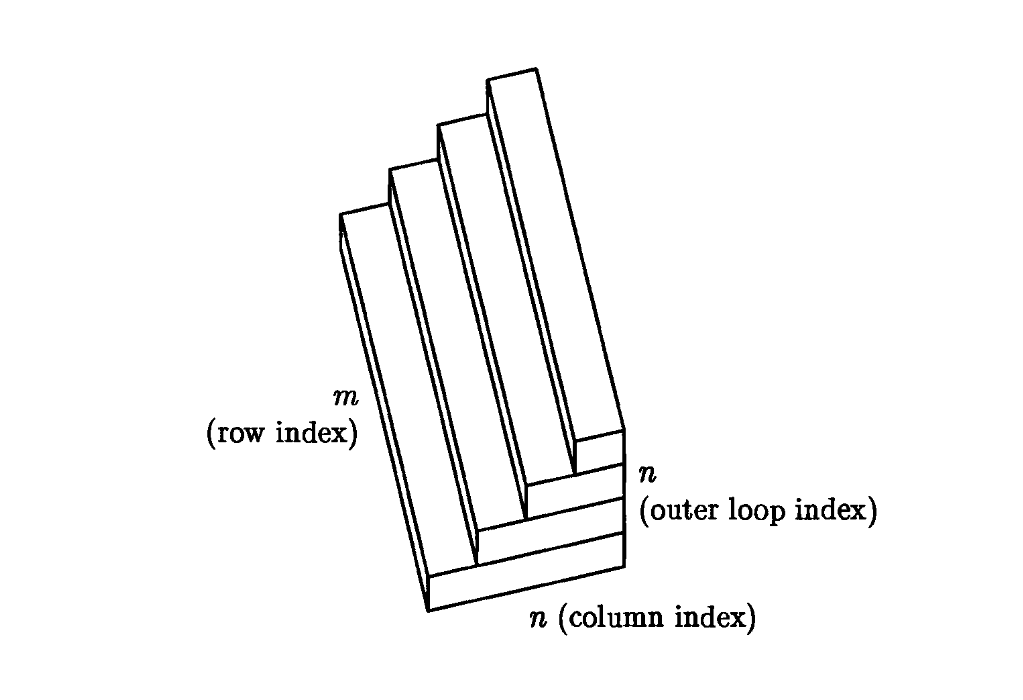
\includegraphics[width=0.8\textwidth]{figures/8-1.png}
\end{figure}
%────────────────────────────────────────
To leading order as $m, n \rightarrow \infty$, then, the operation count for GramSchmidt orthogonalization is proportional to the volume of the figure above. The constant of proportionality is four flops, because as noted above, the two steps of the inner loop correspond to four operations at each matrix location. Now as $m, n \rightarrow \infty$, the figure converges to a right triangular prism, with volume $m n^2 / 2$. Multiplying by four flops per unit volume gives, again,
Work for Gram-Schmidt orthogonalization: $\sim 2 m n^2$ flops.

\section{Gram-Schmidt as Triangular Orthogonalization}
Each outer step of the modified Gram-Schmidt algorithm can be interpreted as a right-multiplication by a square upper-triangular matrix. For example, beginning with $A$, the first iteration multiplies the first column $a_1$ by $1 / r_{11}$ and then subtracts $r_{1 j}$ times the result from each of the remaining columns $a_j$. This is equivalent to right-multiplication by a matrix $R_1$ :
%────────────────────────────────────────
\begin{figure}[H]
    \centering
    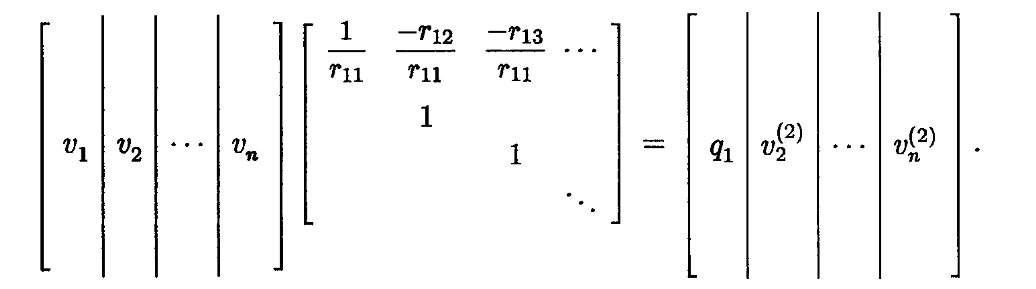
\includegraphics[width=0.8\textwidth]{figures/8-2.png}
\end{figure}
%────────────────────────────────────────
In general, step $i$ of Algorithm~\ref{Algo 8.1} subtracts $r_{i j} / r_{i i}$ times column $i$ of the current $A$ from columns $j>i$ and replaces column $i$ by $1 / r_{i i}$ times itself. This corresponds to multiplication by an upper-triangular matrix $R_i$ :
\[
    R_2 = \begin{bmatrix}[] 
        1 &  &  &   \\
         & \frac{1}{r_{ 22 } } & -\frac{r_{23}}{r_{22}} &  \cdots \\
         &  & 1 &   \\
         &  &  & \ddots  \\
    \end{bmatrix}, \quad R_3 = \begin{bmatrix}[] 
         1&  &  &   \\
         &1  &  &   \\
         &  &\frac{1}{r_{ 33 } }    &\cdots   \\
         &  &  &  \ddots \\
    \end{bmatrix} , \ldots . 
\]

At the end of the iteration we have
\begin{align*}
A \underbrace{R_1 R_2 \cdots R_n}_{\hat{R}^{-1}}=\hat{Q} .
\end{align*}
This formulation demonstrates that the Gram-Schmidt algorithm is a method of triangular orthogonalization. It applies triangular operations on the right of a matrix to reduce it to a matrix with orthonormal columns. Of course, in practice, we do not form the matrices $R_i$ and multiply them together explicitly. The purpose of mentioning them is to give insight into the structure of the Gram-Schmidt algorithm. In Chapter 19 we shall see that it bears a close resemblance to the structure of Gaussian elimination.